\documentclass[handout,nooutcomes]{ximera}
%% handout
%% space
%% newpage
%% numbers
%% nooutcomes

%I added the commands here so that I would't have to keep looking them up
%\newcommand{\RR}{\mathbb R}
%\renewcommand{\d}{\,d}
%\newcommand{\dd}[2][]{\frac{d #1}{d #2}}
%\renewcommand{\l}{\ell}
%\newcommand{\ddx}{\frac{d}{dx}}
%\everymath{\displaystyle}
%\newcommand{\dfn}{\textbf}
%\newcommand{\eval}[1]{\bigg[ #1 \bigg]}

%\begin{image}
%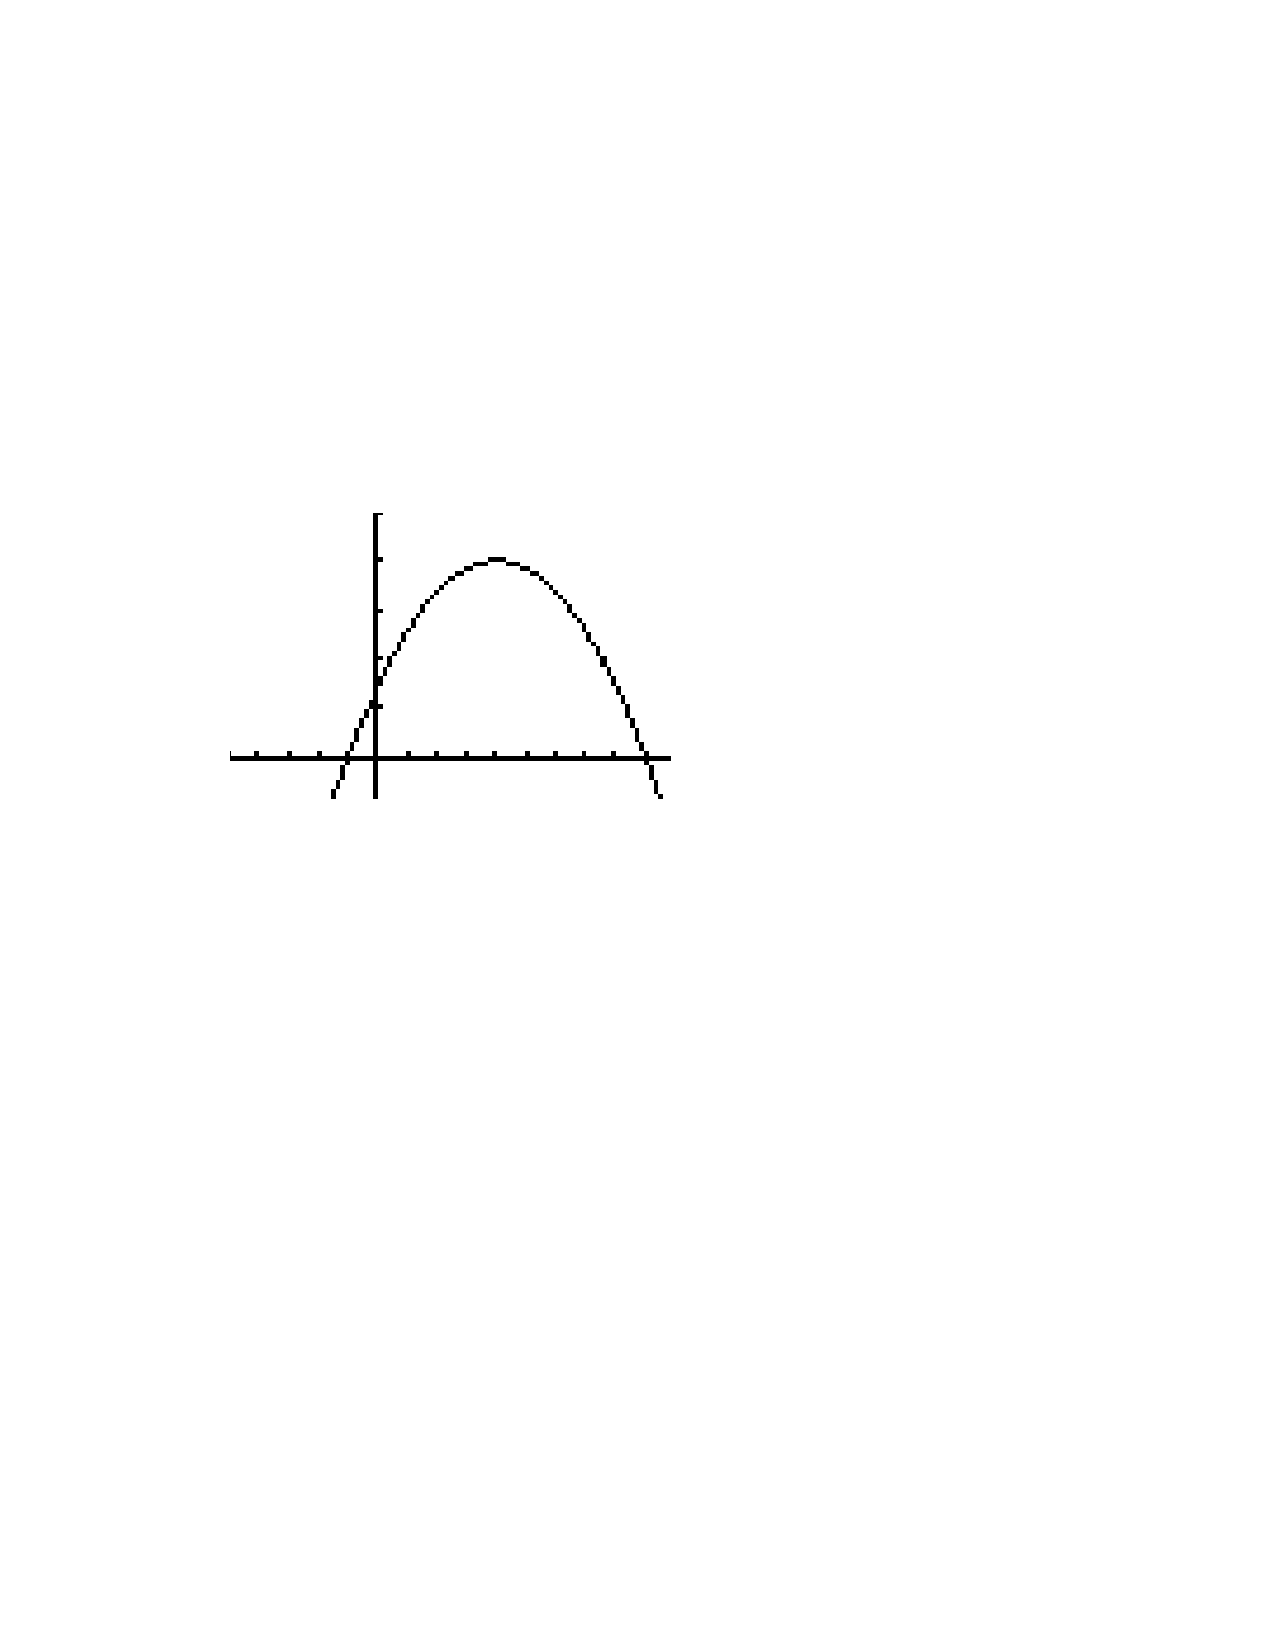
\includegraphics[trim= 170 420 250 180]{Figure1.pdf}
%\end{image}


\newcommand{\RR}{\mathbb R}
\renewcommand{\d}{\,d}
\newcommand{\dd}[2][]{\frac{d #1}{d #2}}
\renewcommand{\l}{\ell}
\newcommand{\ddx}{\frac{d}{dx}}
\newcommand{\dfn}{\textbf}
\newcommand{\eval}[1]{\bigg[ #1 \bigg]}

\usepackage{multicol}

\renewenvironment{freeResponse}{
\ifhandout\setbox0\vbox\bgroup\else
\begin{trivlist}\item[\hskip \labelsep\bfseries Solution:\hspace{2ex}]
\fi}
{\ifhandout\egroup\else
\end{trivlist}
\fi} %% we can turn off input when making a master document

\title{Recitation \#22 - 5.1 Approximating Areas Under Curves}  

\begin{document}
\begin{abstract}		\end{abstract}
\maketitle

\section{Warm up:} 
If a function is positive and decreasing on an interval $[a,b]$, will a right Riemann sum underestimate or overestimate the area of the region under the graph of the function? Justify your answer.
		\begin{freeResponse}
		Because the function is decreasing, a right Reimann sum will be an underestimate.  By definition, $f(x_k)< f(x)$ for all $x$ in the interval $[x_{k-1},x_k]$ 
		\end{freeResponse}	
		
		
		

	
	
	
	
	

\section{Group work:}



%problem 1
\begin{problem}
Snow is accumulating on the ground at a rate of  
$$f^\prime (t)=1.5t-.25 t^2+.3$$
inches per hour for $t$ in $[0,4]$ (i.e., the snow falls for 4 hours- from noon until 4PM).  

There were already $5$ inches of snow on the ground when the storm started.  What does this statement say notation-wise?

A natural question would be to ask how much the amount of snow on the ground changed during the storm.  But because the rate is always changing, this is a difficult question to answer (yet, we will eventually answer it!).  Let’s take what we know about constant rates and amounts and use that to help us answer our question (i.e., once again, taking what we know and using it to find out something about what we do not know).

	\begin{enumerate}
	
	%part a
	\item  Assume the rate stays the same as it was at the start of the storm: 0.3 inches per hour.  How much did the height of the snow on the ground change?  Is this a realistic estimate?
		\begin{freeResponse}
		We are assuming that snow is falling at a constant rate of $f^\prime (0)=.3$ inches per hour for the full four hours.  We estimate that the net amount of snow fallen is:
		
		  (rate snow is falling)$\times$(change in time)=$f^\prime (0) \cdot (4-0) =.3 \cdot 4=1.2$ inches of snow.  
		  
		  No this is not a realistic estimate because $f^\prime$ is not constant.
		\end{freeResponse}
		
		
		
	%part b
	\item  Now assume the rate is the same as it is at the start for the first two hours, then changes to what it is at 2PM for the final two hours.  How much did the height of the snow on the ground change?  Is this a realistic estimate?  Is it likely to be better or worse than that of part (a)?
		\begin{freeResponse}
		We are assuming that snow is falling at a constant rate of $f^\prime (0)=.3$ inches per hour for the first two hours, then at the constant rate of $f^\prime (2)=2.3$ inches per hour for the final two hours.  Thus, we estimate that the net amount of snow fallen is:
		
		  $f^\prime (0)\cdot (2-0)+ f^\prime (2) \cdot (4-2)= (0.3)(2) + (2.3)(2) = 0.6+4.6=5.2$ inches.
		  
		   No this is not a realistic estimate, but it is better than the estimate from part (a).  
		\end{freeResponse}
		
		
		
	%part c
	\item  Now assume the rate stays constant by the hour (i.e., it only changes on the hour to its rate at those times of noon, 1PM, 2PM, and 3PM).  How much did the height of the snow change?
		\begin{freeResponse}
		We are assuming that snow is falling at a constant rate of $f^\prime (0)=.3$ inches per hour for the first hour, then at the constant rate of $f^\prime (1)=1.55$ inches per hour for the second hour, then at a constant rate of $f^\prime (2)=2.3$ inches per hour for the third hour, and finally at a constant rate of $f^\prime (3)=2.55$ inches per hour for the final hour.  c. Thus, we estimate that the net amount of snow fallen is:
		$$ (0.3)(1) + (1.55)(1) + (2.3)(1) + (2.55)(1) = 0.3 + 1.55 + 2.3 + 2.55 = 6.7 $$
		
		So we estimate that 6.7 inches of snow fell throughout the four hours.
		\end{freeResponse}
		
		
		
	%part d
	\item  Now do the same, but it changes on the half-hour.
		\begin{freeResponse}
		Snow falls at the constant rate of $f^\prime (0)=.3$ inches per hour for the first half hour, then at the constant rate of $f^\prime (.5)=.9875$ inches per hour for the next half hour, then at the constant rate of $f^\prime (1)=1.55$ inches per hour for the next half hour, and so on, changing rates at each half hour to the constant rates of $f^\prime (1.5)=1.9875, f^\prime (2)=2.3, f^\prime (2.5)=2.4875, f^\prime (3)=2.55, $ and $f^\prime (3.5)=2.4875$ inches per hour, respectively.  Thus, we estimate that the net amount of snow fallen is:
		\begin{align*}
		& [0.3 + 0.9875 + 1.55 + 1.9875 + 2.3 + 2.4875 + 2.55 + 2.4875](0.5) \\
		&= 7.325 \text{ inches}.
		\end{align*}
		\end{freeResponse}
		
		
		
	%part e
	\item  What would we need to do to find the exact amount that the height of the snow on the ground changed?  And how much snow in total would be on the ground?  Describe these in words, do not try to calculate them.
		\begin{freeResponse}
		To find the exact amount of snow that fell, we would need to calculate the amount of snow that fell at $n$ different places, add them up, multiply by $\frac{4}{n}$, and then take the limit at $n$ goes to infinity.
		\end{freeResponse}
		
		
		
	\end{enumerate}
		
		
\end{problem}
















%problem 2
\begin{problem}
Estimate the area under each curve with the given value of $n$ using a right Riemann Sum. Write the sum in summation notation.
	\begin{enumerate}
	%part a
	\item  $f(x) = x^2 - 9x + 18$, \; $[7,10]$, \; $n=6$
		\begin{freeResponse}
		$\Delta x=\frac{b-a}{n}=\frac{10-7}{6}=\frac{1}{2}.$  \\
		$x_i =a+i\Delta x=7+\frac{1}{2}i.$  
		\begin{align*}
		\sum_{i=1}^{6} f(a + i \Delta x) \Delta x &= \sum_{i=1}^{6} \left( f \left( 7 + \frac{1}{2} i \right) \cdot \frac{1}{2} \right)  \\
		&= \frac{1}{2} \sum_{i=1}^{6} \left( \left( 7 + \frac{1}{2} i \right)^2 - 9 \left( 7 + \frac{1}{2} i \right) + 18 \right) \\
		&= \frac{1}{2} \sum_{i=1}^{6} \left( 49 + 7i + \frac{1}{4} i^2 - 63 - \frac{9}{2} i + 18 \right) \\
		&= \frac{1}{2} \sum_{i=1}^{6} \left( 4 + \frac{5}{2} i + \frac{1}{4} i^2 \right) \\
		&= \frac{1}{2} \left( 4 \sum_{i=1}^{6} 1 + \frac{5}{2} \sum_{i=1}^{6} i + \frac{1}{4} \sum_{i=1}^{6} i^2 \right) \\
		&= \frac{1}{2} \left( 4(6) + \frac{5}{2} \cdot \frac{(6)(7)}{2} + \frac{1}{4} \cdot \frac{(6)(7)(13)}{6} \right) \\
		&= \frac{1}{2} \left( 24 + \frac{105}{2} + \frac{91}{4} \right) \\
		&= \frac{1}{2} \cdot \frac{96 + 210 + 91}{4} = \frac{397}{8}
		\end{align*}
		\end{freeResponse}
		
		
		
	%part b
	\item  $\sin (x)$, \; $\left[ 0, \frac{\pi}{2} \right]$, \; $n=3$
		\begin{freeResponse}
		$\Delta x=\frac{b-a}{n}=\frac{\frac{\pi }{2}-0}{3}=\frac{\pi }{6}$.  \\
		$x_i=a+i\Delta x=0+\frac{\pi }{6}i=\frac{\pi }{6}i.$
		\begin{align*}
		\sum_{i=1}^{3}  f ( a + i \Delta x ) \Delta x  &= \sum_{i=1}^{3} \left( f \left( \frac{\pi}{6}i \right) \cdot \frac{\pi}{6} \right) \\
		&= \frac{\pi}{6} \sum_{i=1}^{3} \sin \left( \frac{\pi}{6} i \right) \\
		&= \frac{\pi}{6} \left( \sin \left( \frac{\pi}{6} \right) + \sin \left( \frac{2 \pi}{6} \right) + \sin \left( \frac{3 \pi}{6} \right) \right) \\
		&= \frac{\pi}{6} \left( \sin \left( \frac{\pi}{6} \right) + \sin \left( \frac{\pi}{3} \right) + \sin \left( \frac{\pi}{2} \right) \right) \\
		&= \frac{\pi}{6} \left( \frac{1}{2} + \frac{\sqrt{3}}{2} + 1 \right)  \\
		&= \frac{\pi}{6} \left( \frac{3}{2} + \frac{\sqrt{3}}{2} \right)  \\
		&= \frac{\pi}{12} (3 + \sqrt{3} )
		\end{align*}
		\end{freeResponse}
		
		
		
	\end{enumerate}
		
		
		

\end{problem}
	
	
	
	
	
	
	
	
			
			






	
	
	
	
	
	
	
	
	

	










								
				
				
	














\end{document} 


















